\documentclass[tikz,border=2pt]{standalone}
\usepackage{amsmath,amssymb}
\usepackage{pgfplots}
\pgfplotsset{compat=1.18}

\begin{document}
% The Bernoulli(p) pmf: all mass on the two outcomes 0 (failure, prob 1-p) and 1 (success,
% prob p); here p = 0.3.
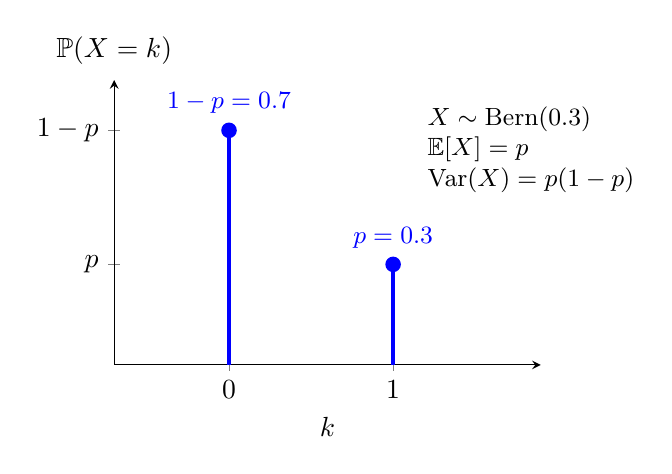
\begin{tikzpicture}
	\begin{axis}[
		axis lines=left, xmin=-0.7, xmax=1.9, ymin=0, ymax=0.85,
		xtick={0,1}, ytick={0.3,0.7}, yticklabels={$p$,$1-p$},
		xlabel={$k$}, ylabel={$\mathbb{P}(X=k)$}, ylabel style={rotate=-90, anchor=south, at={(axis description cs:0,1.02)}},
		width=7cm, height=5.2cm, clip=false
		]
		\addplot[ycomb, blue, very thick, mark=*, mark size=2.2pt] coordinates {(0,0.7) (1,0.3)};
		\node[blue, anchor=south, font=\small] at (axis cs:0,0.72) {$1-p=0.7$};
		\node[blue, anchor=south, font=\small] at (axis cs:1,0.32) {$p=0.3$};
		\node[anchor=north west, font=\small, align=left] at (axis cs:1.15,0.8) {$X\sim\operatorname{Bern}(0.3)$\\ $\mathbb{E}[X]=p$\\ $\operatorname{Var}(X)=p(1-p)$};
	\end{axis}
\end{tikzpicture}
\end{document}
